\documentclass{article}
\usepackage[utf8]{inputenc}
\usepackage[english]{babel}
\usepackage{hyperref}
\usepackage{graphicx}

\hypersetup{
    colorlinks=true,
    linkcolor=blue,
    filecolor=magenta,      
    urlcolor=blue,
}

\title{Assistive Web Tools and Accessibility Standards}
\author{}
\date{}

\begin{document}

\maketitle

\section{Assistive Web Tools}

Assistive web tools encompass a broad range of software applications, browser extensions, specialized hardware devices, and operating system accessibility features. These technologies aim to eliminate digital barriers and provide equal access to web applications, media, and services for individuals with visual, auditory, physical, or cognitive impairments. Following global web accessibility standards like the Web Content Accessibility Guidelines (WCAG) ensures these tools interface effectively with modern websites.

\begin{figure}[h!]
    \centering
    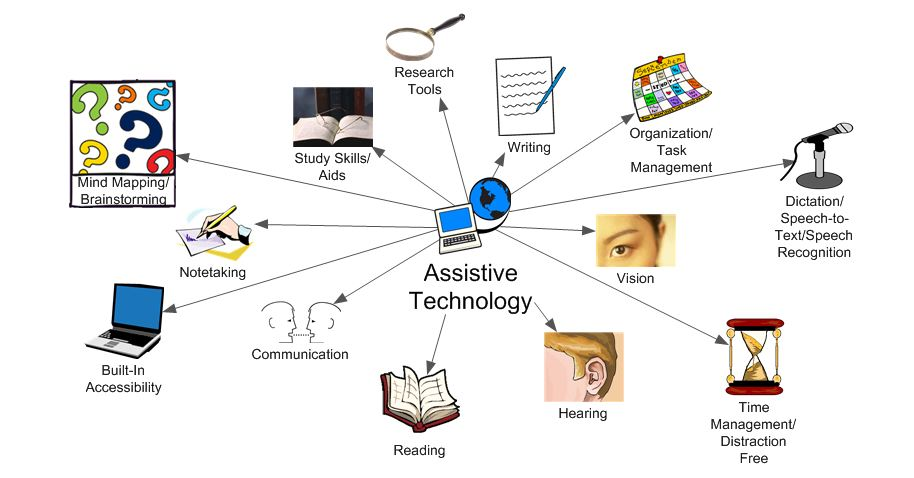
\includegraphics[width=0.8\textwidth]{AT-Mind-Map-for-Website.jpg}
    \caption{Assistive Technology Mind Map for Web}
\end{figure}

\section{Screen Readers}

Screen readers are essential software applications designed to translate digital visual information into synthesized speech or tactile Braille displays. They interact directly with browser accessibility APIs and the Document Object Model (DOM) rather than analyzing the visual layout. Popular implementations include NVDA, JAWS, Apple VoiceOver, and Google TalkBack. 

Developers support screen readers by implementing native semantic HTML elements (\texttt{<nav>}, \texttt{<main>}, \texttt{<button>}), providing precise image \texttt{alt} text, configuring WAI-ARIA attributes (\texttt{aria-expanded}, \texttt{aria-label}), and defining \texttt{aria-live} regions for dynamic content updates.

\begin{figure}[h!]
    \centering
    \includegraphics[width=0.8\textwidth]{1*cYOB76MZE6DNDBlwNrsUvQ.jpg}
    \caption{Screen Reader User Interaction}
\end{figure}

\section{Magnifiers}

Screen magnifiers enlarge visual content on a digital display, assisting individuals with low vision, visual fatigue, or partial sight impairments. Modern magnification software provides adaptive zoom levels, continuous cursor and focus tracking, customizable viewport configurations, high-contrast pointer indicators, and dynamic font smoothing.

Web developers accommodate screen magnifiers by designing flexible, responsive layouts that maintain structure when zoomed up to 400\%. Crucially, layouts must prevent text clipping, overlapping containers, or forced horizontal scrolling at high zoom levels.

\begin{figure}[h!]
    \centering
    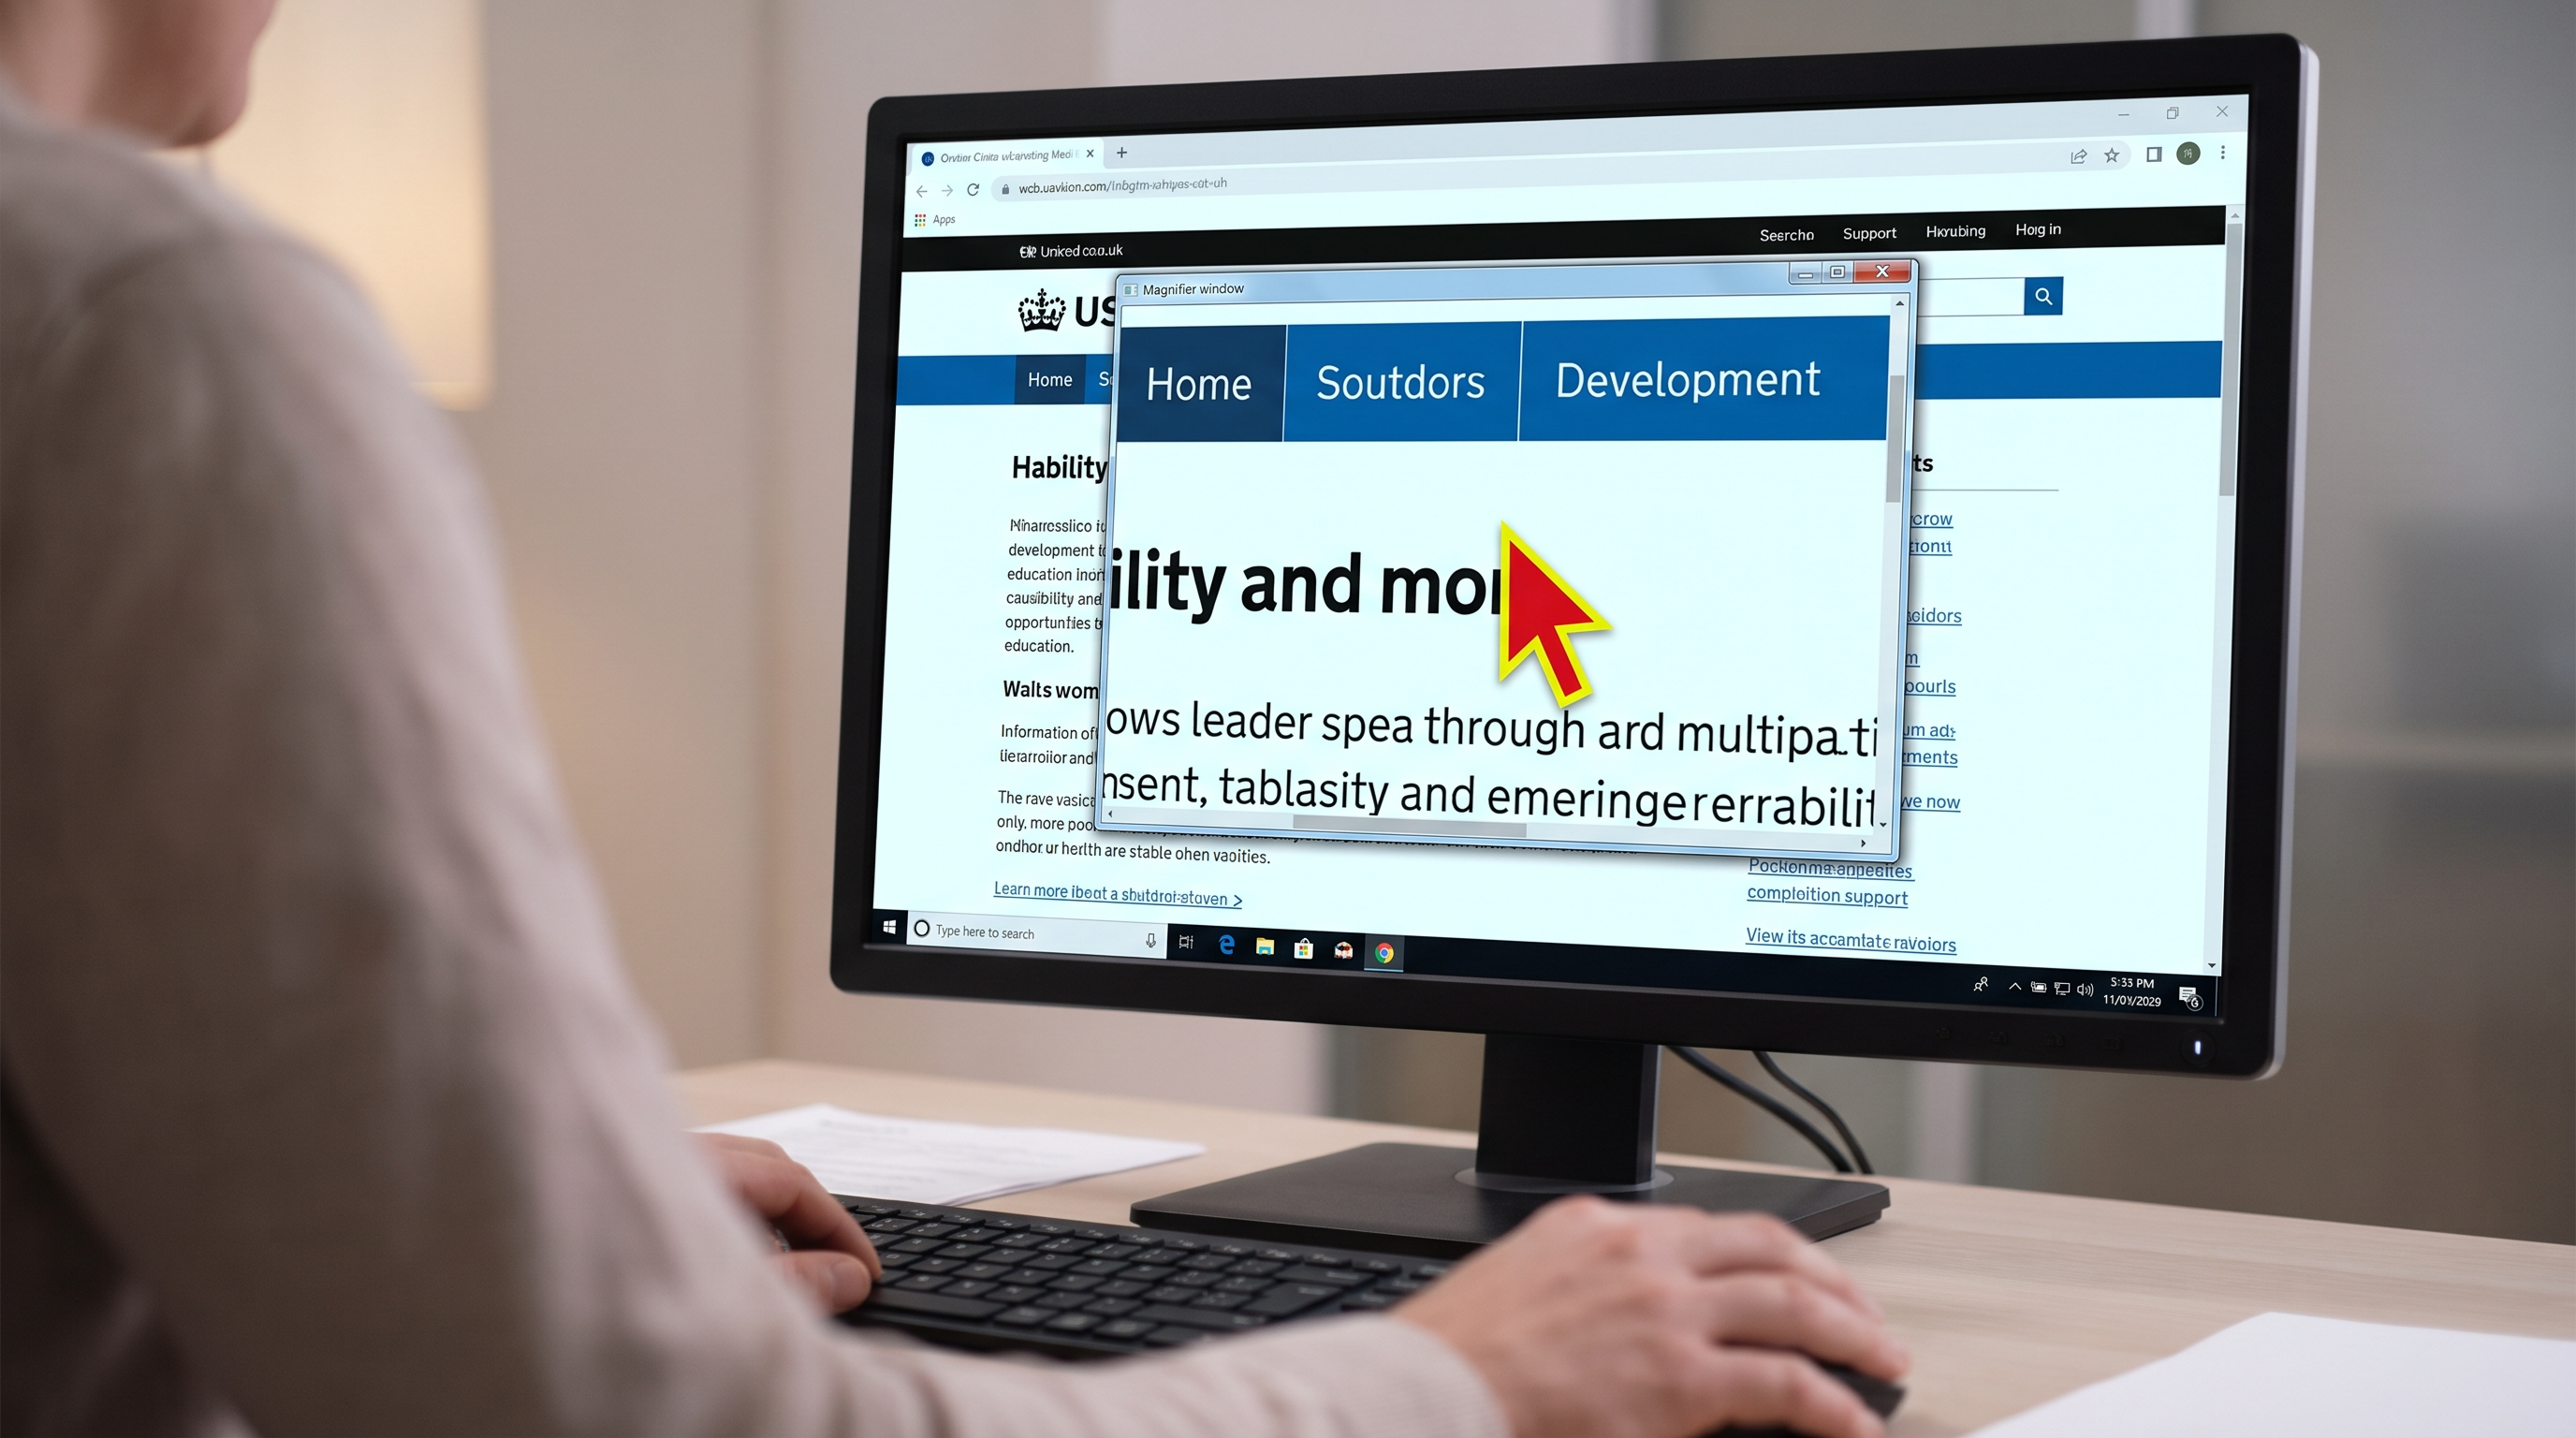
\includegraphics[width=0.8\textwidth]{Magnifiers.jpg}
    \caption{Screen Magnification on a Computer Monitor}
\end{figure}

\section{Keyboard Navigation}

Keyboard navigation enables users to browse and interact with digital interfaces entirely without a physical mouse or touchscreen. This access mode is critical for individuals with fine motor control challenges, tremors, or permanent physical disabilities.

Compliant web interfaces support full keyboard operation using standard keys (\texttt{Tab}, \texttt{Shift+Tab}, \texttt{Enter}, \texttt{Spacebar}, and arrow keys). Key implementation requirements include maintaining a logical DOM tab order, displaying distinct CSS focus rings (\texttt{:focus-visible}), managing focus inside modal dialogs, and providing skip-to-content links.

\section{High Contrast and Custom Color Themes}

High contrast modes and custom color themes adjust visual presentations for users with color blindness, photophobia, low vision, or sensitivity to visual brightness. Developing accessible visual themes requires meeting standard WCAG contrast ratios (such as a minimum of 4.5:1 for standard body text), integrating operating system color modes (e.g., CSS \texttt{forced-colors}), and offering user-selectable dark and light themes.

Furthermore, accessible design dictates that color must never serve as the sole method for conveying information, signaling interactions, or displaying validation errors.

\begin{figure}[h!]
    \centering
    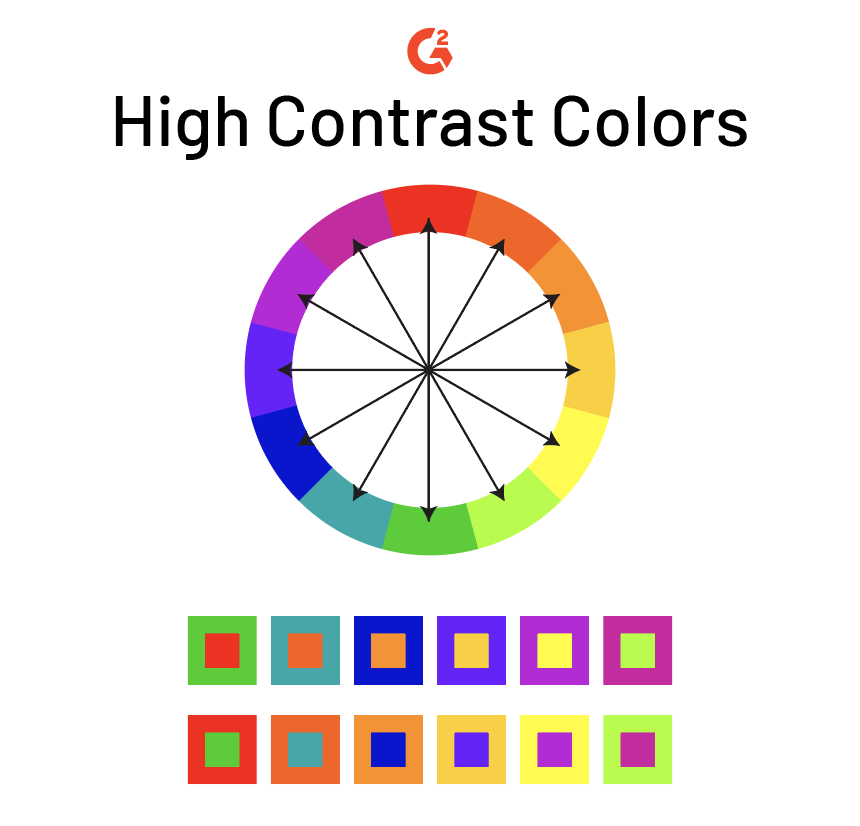
\includegraphics[width=0.4\textwidth]{high contrast colors.png}
    \caption{High Contrast Color Palette}
\end{figure}

\section{Alternative Input and Speech Recognition}

Alternative input methods and speech recognition software enable individuals with severe motor disabilities or limb differences to interact with web interfaces through voice commands, eye-tracking hardware, head pointers, or single-switch devices. Users can issue spoken navigation commands or trigger interface actions through switch cycles.

Designing for alternative input requires large click targets, visible activation labels matching accessible DOM names, avoidance of complex multi-touch gestures, and robust native form elements.

\begin{figure}[h!]
    \centering
    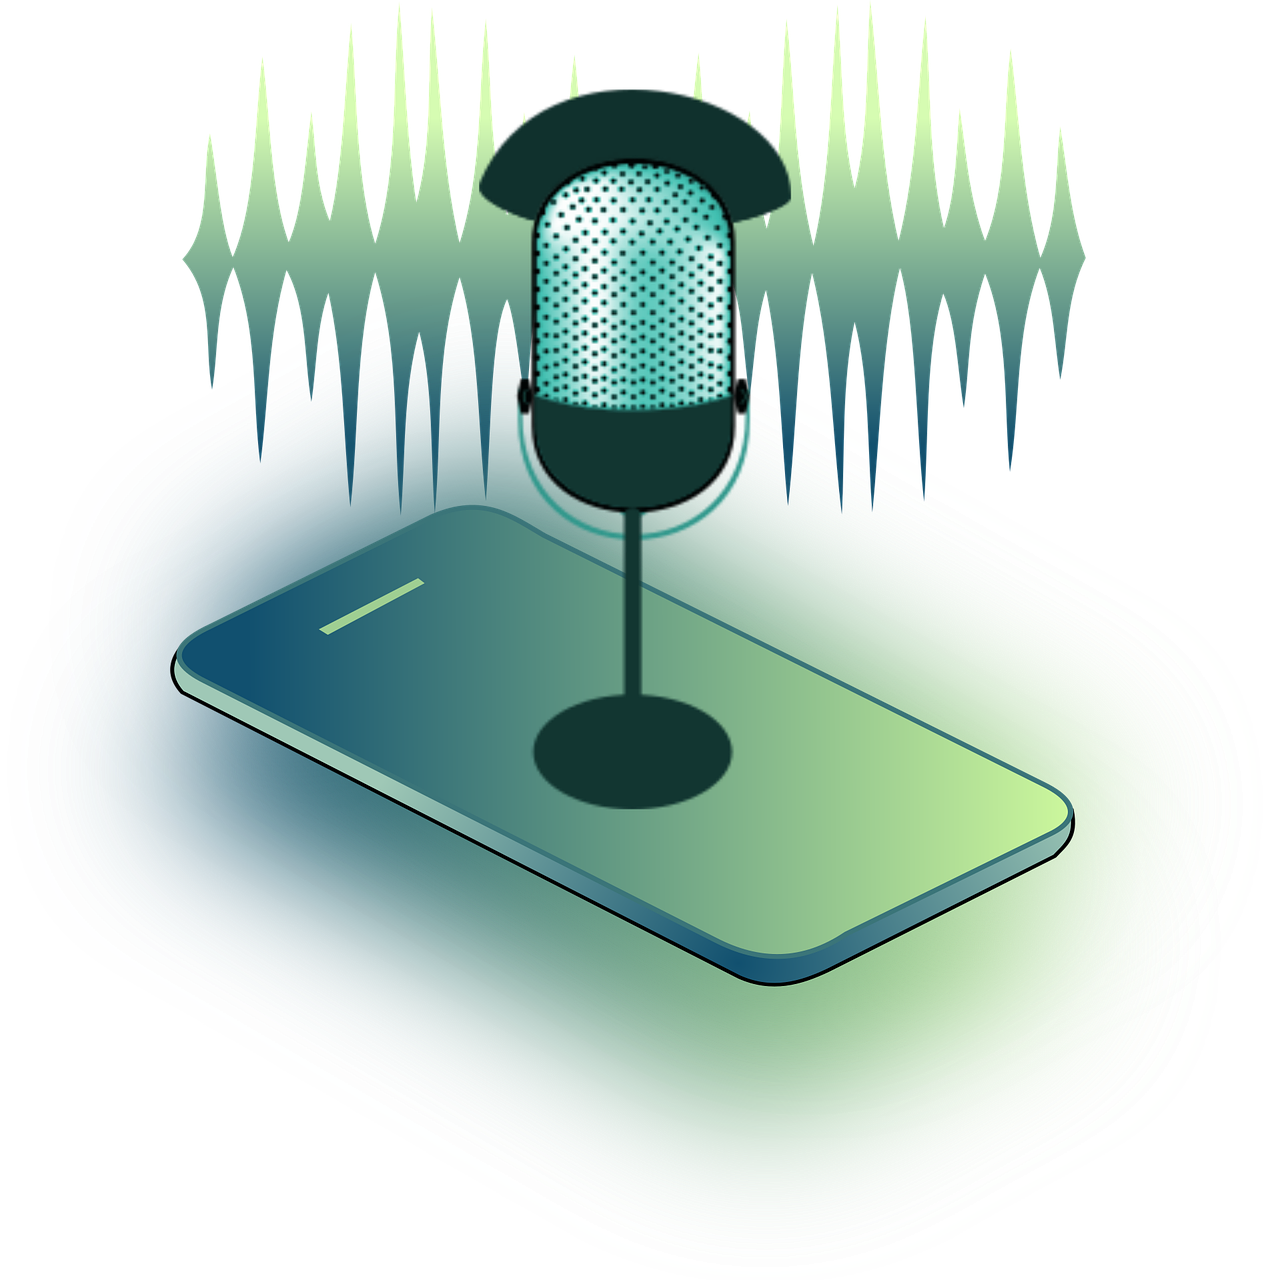
\includegraphics[width=0.4\textwidth]{voicerecog.png}
    \caption{Voice Recognition and Speech Input}
\end{figure}

\section{Links}

\begin{itemize}
    \item \textbf{W3C WAI Home:} \href{https://www.w3.org/WAI/}{W3C Web Accessibility Initiative}
    \item \textbf{W3C How People Use the Web:} \href{https://www.w3.org/WAI/people-use-web/}{W3C: How People with Disabilities Use the Web}
    \item \textbf{Tools and Techniques:} \href{https://www.w3.org/WAI/people-use-web/tools-techniques/presentation/}{W3C WAI: Presentation and Customization Tools}
    \item \textbf{WebAIM Main Resource:} \href{https://webaim.org/}{WebAIM: Web Accessibility in Mind}
    \item \textbf{W3C Perspectives Overview:} \href{https://www.w3.org/WAI/perspective-videos/}{W3C Web Accessibility Perspectives Videos}
\end{itemize}

\end{document}